\documentclass[aps,prl,twocolumn,superscriptaddress,groupedaddress]{revtex4}  
\usepackage{graphicx,float,hyperref}  
\usepackage{dcolumn}   
\usepackage{bm}        
\usepackage{amssymb,lipsum}
\usepackage[spanish]{babel} 
\usepackage[utf8]{inputenc}
\hyphenation{ALPGEN}
\hyphenation{EVTGEN}
\hyphenation{PYTHIA}
\begin{document}
\title{Simulación de Propiedades Mecánicas de Carbono Amorfo}
\affiliation{Universidad Mayor, Santiago, Chile}
\author{Daniel Castillo-Castro} \affiliation{Universidad Mayor, Santiago, Chile}
\author{Rafael González} \affiliation{Universidad Mayor, Santiago, Chile}
     
\date{\today}
\begin{abstract}
El carbono amorfo es un material de reciente interés en ciencia de materiales. Evaluar sus propiedades termodinámicas y mecánicas constituye un paso importante hacia sus aplicaciones. En este trabajo se presenta un estudio de simulación de dinámica molecular clásica en el que comparamos su modelado utilizando diferentes potenciales interatómicos. El estudio se realizó usando varios potenciales interatómicos y las simulaciones de muestras de carbono amorfo a partir de celdas cúbicas sometidas a rampas de temperatura. A estas muestras se les midió punto de cambio de fase a grafito y módulo de bulto, buscando propiedades termodinámicas del material. Se obtuvo temperaturas de cambio de fase en el orden de los 2000~K para diferentes potenciales y módulos de bulto del orden de los 200 a 300~GPa. De todos los potenciales evaluados, EDIP es el de mejor desempeño.
\end{abstract}

\maketitle
En los últimos años, uno de los temas más investigados en el campo de la información cuántica son los Centros de Color de diamante, que consisten en insertar un defecto puntual en un diamante de simetría 3m, sustituyendo carbonos por un nitrógeno y una valencia en la dirección $<111>$.\cite{NVDiamond} Dentro de esa área, un interés de investigación reciente es la realización de centros en los llamados nanodiamantes, que no son otra cosa que secciones pequeñas dentro de un carbono amorfo que tienen la estructura química de un diamante (que contiene enlaces del tipo sp$^3$, a diferencia del grafito que contiene fundamentalmente enlaces sp$^2$). Esto hace al carbono amorfo un material muy interesante de trabajar para los científicos de Óptica e Información Cuántica, tanto teóricos como experimentales.

Más allá de esto, analizar un material termodinámicamente es de interés fundamental. Por otro lado, se ha demostrado una relación directa entre procesos de Información Cuántica y de Termodinámica Cuántica. En principio porque ambas teorías comparten el concepto de entropía, lo que sugiere vínculos entre ambas \cite{QTh} y ha llevado a la realización de estudios sobre flujos de información y sus efectos termodinámicos, por ejemplo, para sistemas de spin. \cite{ThermoQIFlow} Es por esto que el análisis de las propiedades termodinámicas del carbono amorfo resulta un área de investigación de gran interés, ya que los algoritmos para obtener dichas propiedades pueden ser interpretados como procesos informáticos de manera análoga a lo que se reporta en literatura. Considerando algunos alótropos de carbono como casos límites y, de manera análoga a como se ha hecho con otros materiales, usando métodos numéricos-computacionales \cite{ThermoFlow}. 

A grandes rasgos, para la unidad de investigación se ocupará dinámica molecular clásica, que consiste en la representación numérica de la interacción y evolución temporal de un arreglo de átomos siguiendo las leyes de Newton.  para generar la evolución temporal de un sistema recursivamente. Exige definir una muestra atómica con todos los parámetros iniciales, es decir, la estructura del sistema atómico y sus velocidades iniciales. Llevar a cabo una simulación de dinámica molecular clásica implica definir potenciales interatómicos que incluyen, aproximadamente, los efectos cuánticos y mediciones experimentales. Uno de los  potenciales más sencillos es el de Lennard-Jones \cite{LJ}, aunque cada vez se ha sofisticado más el desarrollo de potenciales para materiales específicos. En términos básicos, un "potencial" es un archivo de texto que contiene cifras que representan parámetros que simularán aproximadamente la interacción entre los átomos. \cite{MDErcolessi} Con simulaciones de dinámica molecular clásica se pueden calcular espectros vibracionales y relacionarlos con mediciones experimentales. Pero se debe ser cuidadoso en la interpretación de estos resultados y recomendable comparar los mismos con resultados con teorías más precisas, por ejemplo, DFT (Teoría de Funcional de Densidad, por sus siglas en inglés), que incluye efectos cuánticos y la estructura electrónica. De todas formas, para el análisis realizado en este trabajo, la simulación de dinámica molecular clásica será de gran interés.

Dicho lo anterior, Marks\cite{ACPot1} propuso un método para obtener muestras de carbono amorfo a partir de un arreglo cúbico de átomos de carbono, en el  cual la distancia interatómica puede hacer variar el porcentaje de enlaces sp$^3$ (es decir, los posibles sectores en los que se comporta como diamante) que terminará teniendo la muestra. Mientras menor sea la distancia interatómica inicial (mayor densidad), mayor porcentaje de enlace sp$^3$ habrá luego del proceso (lo que significa que el carbono amorfo será más cercano al diamante). El método consiste en  calentar la muestra hasta $10000$~K en $0.25$~ps (pico-segundos) y enfriarse en un proceso lento de 5~ps. A continuación, para poder medir propiedades termodinámicas, se realizó una simulación en condiciones NPT aún más lento de 25~ps. Debemos que considerar que las variables del sistema, como temperatura y presión, en dinámica molecular clásica se calculan como un promedios temporales de las  propiedades de las átomos en el sistema. Por lo que para que las propiedades den valores más precisos es mejor que estos promedios sean representativos de un sistema que empieza en equilibrio. Una muestra gráfica del proceso se encuentra en la Figura~\ref{fig:carbon}.

Como se mencionó antes, el potencial elegido para realizar esta medición siempre será una aproximación al sistema real. Entonces, habrá mejores aproximaciones que otras para los sistemas de interés. Marks y su equipo han desarrollado el potencial EDIP, que se ajusta muy bien para muestras con alótropos de carbono (esto incluye al carbono amorfo) de acuerdo a investigaciones que han estudiando su comportamiento con respecto a potenciales como REBO o COMB para creación y destrucción de enlaces químicos\cite{ACPot2}. Un procedimiento similar se usará para medir propiedades como cambios de fase en relación a la temperatura y módulos de bulto, tópicos de importancia considerable de acuerdo a lo señalado anteriormente.

    \begin{figure}
        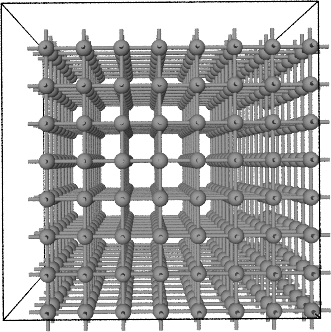
\includegraphics[width=0.3\textwidth]{carbon1.png}\\
        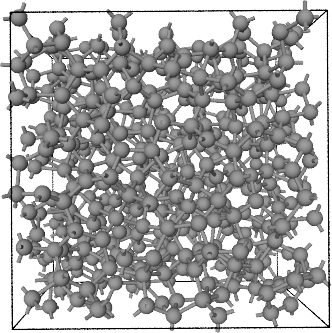
\includegraphics[width=0.3\textwidth]{carbon2.png}
    \label{fig:carbon}
    \caption{El proceso utilizado convierte un arreglo cúbico de átomos de carbono (arriba) en una muestra de carbono amorfo (abajo) con un porcentaje de enlaces sp$^3$ a definir. Para cada potencial y distancia interatómica inicial se producirá un porcentaje de sp$^3$ distinto. }
   \end{figure}

 En la Figura~\ref{fig:meltproc} se muestra el calentamiento de una muestra. El objetivo inicial del desarrollo era encontrar los valores de punto de fusión de carbono amorfo, pero se observa un cambio de fase estructural a grafito estructural, y no de estado sólido-líquido como esperábamos en un principio. Esto está de acuerdo con la derivación sobre las fases del carbono hecha en el LHC (Gran Colisionador de Hadrones de acuerdo a su sigla en inglés), que predice dicho cambio de fase a temperatura alta (entre 2000 y 3000K) y presión atmosférica.\cite{Zazula}  Más allá de eso, lo que se mostrará en este informe son los puntos de cambio de fase (para el cambio recién señalado) y módulos de bulto para el sistema de carbono amorfo. Los módulos de bulto se definen como la resistencia a la compresión del material y que matemáticamente se define como:
 \begin{equation} K=-v\frac{dP}{dV}, \end{equation} donde V es el volumen y P la presión. 
 
 Se trabajó con potenciales mencionados en \cite{ACPot1} como REBO (Potencial de órden de enlace reactivo empírico, incluyendo varias de sus variantes) , BOP (Potencial de orden de enlace), COMB (potencial de muchos cuerpos optimizado en carga), ReaxFF (Campo de fuerza reactivo) y Tersoff (nombrado por su autor), además de EDIP (Potencial interatómico dependiente del ambiente) como referencia, aunque para este informe se seleccionaron los potenciales que entregaron mejores resultados y usaron un tiempo razonable de computación. Se procuró, para seguir la secuencia de generación de carbono amorfo, el cálculo del punto de cambio de fase y el cálculo del módulo de bulto seguir ocupando para cada caso el mismo potencial en toda el proceso descrito antes. Se evaluó, para cada muestra, los porcentajes de enlaces de carbono tipo sp$_3$ usando el programa OVITO (\textit{Open Visualization Tool}, de acuerdo a su sigla en inglés) \cite{Ovito}, tomando las muestras finales y calculando los enlaces entre todos los átomos, tomando como enlazados aquellos átomos a una distancia menor a 2~\AA. 

La medición de los puntos de cambio de fase para todas las muestras se obtuvo observando la dinámica dentro de la muestra a través del programa OVITO, lo que luego se comparó con las gráficas que denotaban un proceso de cambio de fase al producirse un alza repentina de volumen en un intervalo corto de temperatura menor a 200K. En la Figura~\ref{fig:meltdata} aparece dicho proceso graficado. Se evaluó para los potenciales AIREBO (REBO en su variante adaptativa intermolecular), BOP, EDIP, ReaxFF y REBO. En la Figura~4 se observa que los valores de temperatura en que comienza el cambio de fase van bajando a medida que el porcentaje de enlaces tipo sp$^3$ aumenta. Lo anterior se puede explicar considerando que mientras la muestra se parece más a un diamante el cambio de fase se empieza a producir a temperatura menor, esto concuerda con el diagrama de fase presentado en el artículo de Zazula~\cite{Zazula}, donde se señala que a presión de una atmósfera  se produce una transición de amorfo a grafito. Se observa en dichas muestras defectos consistentes con enlaces tipo sp$^1$ que desaparecen al cambiar la temperatura y son inestables. 

    \begin{figure}
        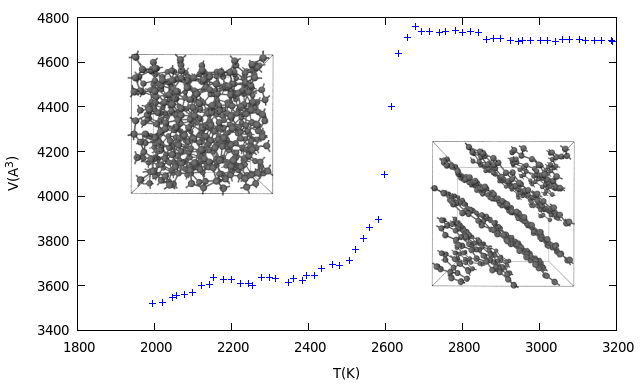
\includegraphics[width=0.5\textwidth]{melting.png}
        \caption{En la figura se muestra el proceso de cambio de fase de amorfo a grafito. La muestra está a presión atmosférica y es sometida a una rampa rápida y a una rampa lenta de temperatura. El gráfico es generado a partir de promediar los resultados en ambas rampas.}
        \label{fig:meltproc}
    \end{figure}
    \begin{figure}
        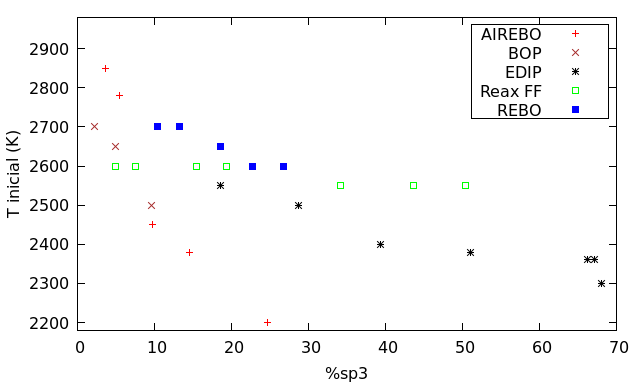
\includegraphics[width=0.5\textwidth]{datamelting.png}\\
        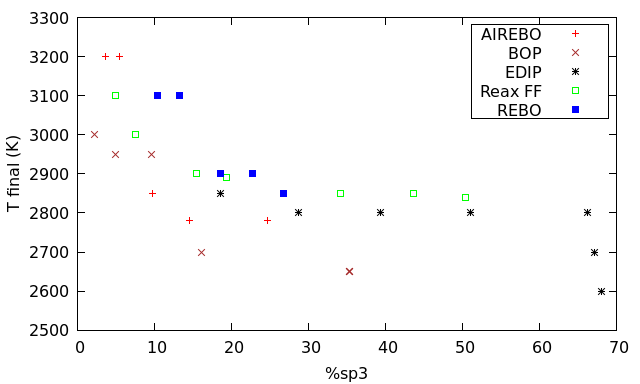
\includegraphics[width=0.5\textwidth]{datameltingfin.png}
        \caption{En el gráfico se muestra tanto la temperatura inicial como la final  de cambio de fase para los potenciales Airebo-m, Bop, Edip, Reax y Rebo. Los ciclos ocurren en ventanas de alrededor de 200~K para luego mantenerse con una estructura tipo grafito hasta 4000~K.}
        \label{fig:meltdata}
    \end{figure}

En cuanto a los valores de módulos de bulto, se obtienen generando archivos que promedian el comportamiento de la muestra al expandirla y contraerla en un intervalo pequeño respecto al largo total. El comportamiento en promedio de la muestra se observa en la Figura~\ref{fig:bulkproc}. En esta figura se muestra una curva que puede aproximarse por una recta (para evaluar dicho ajuste se ocupó el código Gnuplot\cite{Gnuplot}) y su pendiente multiplicada por el volumen inicial de la muestra es el módulo de bulto. Evaluamos este módulo para los potenciales AIREBO, ReaxFF, REBO y EDIP. Se obtienen en las muestras valores entre 100 y 300 GPa Figura~\ref{fig:bulkdata}, lo que concuerda con el trabajo de Ito {\it et al.} que presentan el módulo de bulto para muestras de carbono amorfo dependiendo de la densidad de masa con valores entre los 200 y 350 GPa.~\cite{RefBulk}
    \begin{figure}
        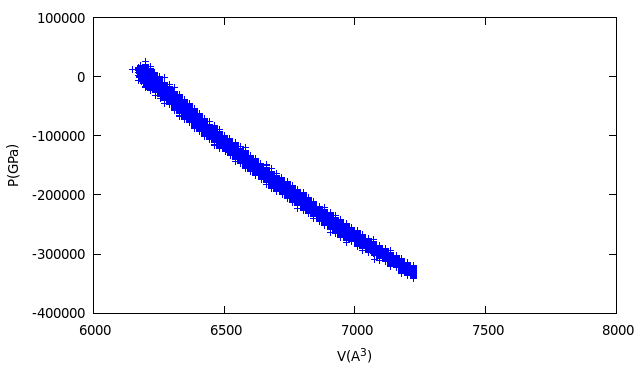
\includegraphics[width=0.5\textwidth]{bulk.png}
        \caption{Respuesta de uno de los casos al algoritmo hecho para calcular módulos de bulto. Consiste en 2 curvas de expansión y contracción de la muestra, aplicándole presión en dirección negativa. El módulo de bulto se obtiene luego de  evaluar la pendiente del ajuste recto de un segmento corto de la expansión.}
        \label{fig:bulkproc}
    \end{figure}
    \begin{figure}
        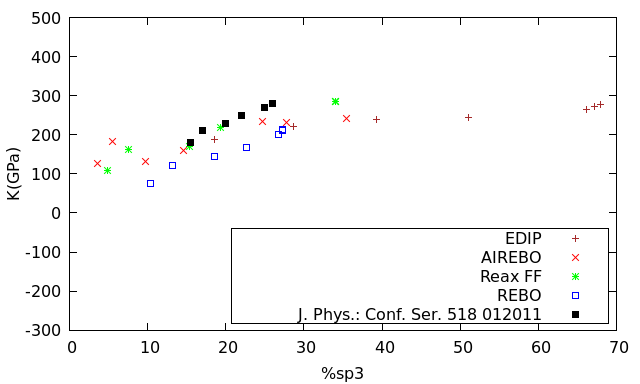
\includegraphics[width=0.5\textwidth]{databulk.png}
        \caption{Gráfico con módulos de bulto para los potenciales Airebo-m, Reax, Rebo y Edip. Se ocupa como referencia \cite{RefBulk}, que evalúa módulos para muestras muy cercanas a diamante. Se observa un comportamiento más ajustado a la referencia para los potenciales airebo-m, rebo y EDIP.}
        \label{fig:bulkdata}
    \end{figure}

Mirando estos resultados, aparece como una pregunta natural por qué los resultados varían respecto a cada potencial. Los potenciales interatómicos se ajustan a distintos tipos de propiedades de la materia.  De acuerdo a lo observado para todos los potenciales evaluados, los datos se ajustan a las mediciones de referencia, al menos aproximadamente, siendo EDIP el que más se acerca. Con lo que se concluye que si se quiere tener resultados con mayor cercanía a los datos que podrían obtenerse con  simulaciones que incluyen efectos cuánticos en muestras de similar tamaño (como por ejemplo la teoría del funciona de densidad o DFT) para variables termodinámicas, una versión adaptada de EDIP podría servir.  

También es necesario recordar que en los cálculos realizados se  trabajó con muestras de 1000 átomos en un arreglo cúbico de alrededor de $1.5$~nm por cada lado de la caja. Esta caja es útil para hacer cálculos de baja demanda computacional, aunque la estadística entregada podría ser insuficiente.  De todas formas, para evaluar una muestra donde se pretende insertar defectos, el tamaño es adecuado (Siguiendo a la literatura que estudia cómo se comportarían los centros de color en muestras similares \cite{NVDiamond}). Otra observación es que en las evaluaciones hechas, tanto para los puntos de cambio de fase como de módulo de bulto, se asocia cada valor obtenido con el porcentaje de enlace sp$^3$ que tiene la muestra al empezar el proceso. Esto lleva a indicar que la información obtenida puede no ser suficiente para obtener una adecuada relación entre el porcentaje de enlaces tipo sp$^3$ y variables termodinámicas. De todas formas, nuestro trabajo es  un buen punto de partida.

La investigación usando métodos numéricos de muestras de carbono amorfo es un campo incipiente y este desarrollo es solo el comienzo de un trabajo que puede crecer más. Posibles proyecciones para trabajos futuros de la simulación serían insertarle defectos propios de un centro de color en nanodiamantes en amorfos con un gran porcentaje de sp$^3$. A la vez, volver a evaluar sus propiedades termodinámicas, sus propiedades vibracionales (existen formas de evaluar con espectroscopia Ramman en este sistema usando LAMMPS y programas  escritos en Python \cite{Phonopy}) y evaluar dichos sistemas usando formalismos más sofisticados como DFT, siempre que los tiempos de computación sean similares al de esta experiencia.\\ 

\begin{thebibliography}{99}
\bibitem{NVDiamond} J.Narayan, A.Bhaumik, Matter.Res.lett 5,NO.4,242–250 (2017).
\bibitem{QTh} J. Goold, M. Huber, A. Riera, L. Del Río, P. Skrzypczyk, J. Phys. 49,14 (2016)
\bibitem{ThermoQIFlow} K. Ptaszyński, M. Espósito, PRL 122,150603 (2019).
\bibitem{ThermoFlow} S. Boucetta , J. Magnesium and Alloys 2,59e63 (2014). 
\bibitem{LJ} J.E. Lennard-Jones, Proc.R.Soc.Lond. A 106,(738):463–477 (1924) 
\bibitem{MDErcolessi} F. Ercolessi, Spring School in Computational Physics, ICTP, Trieste (1997).
\bibitem{ACPot1} C. De Tomás, I. Suarez-Martínez ,N. Marks, Carbon 109,681-693 (2016).
\bibitem{ACPot2} E. Tangarife ,R. González, Cardenas C, Bringa E.M., Muñoz F., Carbon 144,177-184 (2019).
\bibitem{Zazula} J. M. Zazula, LHC Project Note 87 (1997)
\bibitem{Lammps} S. Plimpton, J Comp Phys 117, 1-19 (1995).
\bibitem{Ovito} A. Stukowski, Matter. Sci. Eng. 18, 015012 (2010)
\bibitem{Gnuplot} T. Williams, C. Kelley [Online] \href{http://www.gnuplot.info/docs_5.3/gnuplot.pdf}{gnuplot.info} (2018)
\bibitem{RefBulk} A. M. Ito, A. Takayama, Y. Oda, H. Nakamura, J. Phys.: Conf. Ser. 518, 012011 (2014)
\bibitem{Phonopy} A. Togo, Scripta Materialia 108, 1-5 (2015)
\end{thebibliography}
\end{document}

